\subsection{Elektrische Konstruktion}
Unser CanSat besteht aus mehreren Sensoren und einem zentralen Verarbeitungssystem sowie einem Sender. Diese kommunizieren alle über verschiedene Protokolle. Im Anhang unter der Einleitung befindet sich das Blockdiagramm unseres Satelliten. Im Blockdiagramm fehlen allerdings die verschiedenen Protokolle, in unserem Fall kommuniziert der BeagleBone Black, die MCU, mit allen Sensoren und holt deren Daten ab.

\begin{table}[H]
  \centering
    \begin{tabular}{rr}
    \toprule
    \textbf{Bauteil} & \textbf{Kommunikationsprotokoll} \\
    \midrule 
    UV ML8511 & ADC \\
    Sharp Feinstaubsensor & ADC \\
    APC220 & UART \\
    Ultimate GPS & UART \\
    TMP006 & I²C \\
    BMP180 & I²C \\
    \bottomrule
    \end{tabular}
    \caption{Kommunikationsprotokolle}
\end{table}

\subsubsection{Fachliche Grundlagen}
\paragraph{Embedded System}
Ein Embedded System ist in unserem Fall der BeagleBone Black. Das Mikrokontrollerboard taktet mithilfe eines ARM Cortex-A6 Prozessors mit 1Ghz. Auf ihm ist der leicht modifizierter Linux Kernel Angstrom mit Frontend installiert. Andere Beispiele für ein Embedded System sind etwa ein Smart TV oder ein Router. Beide besitzen eine Main Control Unit mit einem Betriebssystem, welches auf die Anwendung des Gerätes spezialisiert ist. In unserem Fall der BeagleBone, welcher verschiedene Technologien besitzt um mit einzelnen Bauteilen zu kommunizieren. UART, I-2-C, SPI, Analog, Digital, PWM, Timer, PRU, ADC, DAC und viele mehr. Viele dieser Technologien sind in unserem Projekt nicht in Verwendung. Jene, die in Verwendung sind, werden später im Dokument beschrieben.

\paragraph{Transistor-Transistor-Logik}
5V werden immer als logisch ``Ein'' bezeichnet. Damit ist gemeint, dass der Sensor, wenn er den höchsten Messwert erreicht, eine Spannung von 5V ausgibt. Ist dies nicht der Fall hat der Sensor eine andere Kennkurve die zum Beispiel bei 3.3V aufhört. Allgemein wird aber die Transistor-Transistor-Logik genutzt, welche 5V als logisch ``Ein'' und geerdet als logisch ``Aus'' ansieht. Es gibt natürlich Toleranzen, welche aber bei verschiedenen integrierte Schaltkreisen und Mikrokontrollern unterschiedlich sind.

\paragraph{Analog-to-Digital-Converter}
Andere Sensoren, beispielsweise der UV-Sensor, verfügen lediglich über einen internen Wiederstand. Der Wiederstand verändert sich in Abhängigkeit zu einer mathematischen Kurve. Dadurch entstehen unterschiedliche Spannungen, welche über den jeweiligen analogen Pin ausgegeben werden. Mithilfe eines Analog-to-Digital-Converter konvertieren wir das analoge Signal, zum Beispiel 5V, in das äquivalente digitale Signal mit einer Auflösung von 12 Bits. \\

\[
2^{12} \quad = 4096
\]

So können 4096 verschiedene Stufen dargestellt werden. Da ein analoges Signal theoretisch in unendlich viele Stufen unterteilt werden kann scheinen 4096 Stufen auf den ersten Blick nicht viel. Ein einzelner Schritt ist trotzdem im digitalen (12 Bits) sehr klein, was folgende Rechnung zeigt.

\[
\frac{5V}{4096} = 0.001220703125 V
\] \\

Das Ergebnis bedeutet, dass man mit 12 Bit eine 5V Spannung in 0.001220703125V Schritten darstellt kann. Dem Arduino Mega 2560 stehen nur 10 Bits zur Verfügung. Da die Rechnung exponentiell ist verkleinert sich dadurch die Anzahl der Stufen enorm.\\

\[
2^{10} \quad = 1024
\]

\[
\frac{5V}{1024} = 0.0048828125V
\] \\

Wie man an dem Ergebnis sieht, kann das BeagleBone den Wert, der am analogen Pin ankommt, viel genauer darstellen, als der Arduino. 

\paragraph{Universal-Asynchronous-Receiver-Transmitter}
UART ist eine digitale serielle Schnittstelle zum Realisieren von einfachen Kommunikationen zwischen zwei Endpunkten. Die Funktionsweise ist denkbar einfach. Wir nutzen in unserem Satelliten meist eine Baudrate von 9600bps. Baud ist die Schrittgeschwindigkeit oder Symbolrate, also 9600 bits per second. Für UART gibt es wie beim RJ45 Stecker TX und RX, die beim Aufbau einer Kommunikation gekreuzt werden. Dies liegt daran, dass der Transciever des einen Komponenten an den Reciever des anderen angeschlossen werden muss. Und natürlich auch andersherum. Nun wird zwischen vielen verschiedenen Arten von UART unterschieden in unserem Fall die TTL-UART Variante welche die beim Analog-to-Digital-Converter genannten 5V als logisch ``Ein'' bezeichnen. \\

\paragraph{Inter-Integrated-Circuit}
I-2-C ist ein serieller Datenbus der über zwei Kabel mit einer 10-Bit-Adressierung (welcher 1024 Stufen entspricht). Der Bus ist auf eine maximalen Geschwindigkeit von 5 Mbit/s beschränkt, welche für unsere Zwecke jedoch ausreichend ist. Der Sinn des Bussystems ist es, mithilfe von einer Adressen einen Datensatz oder Befehl nur an den gewünschten Empfänger zu senden. I-2-C benötigt lediglich eine Datenleitung, welche den eine Kommunikation zwischen dem Master (in unserem Fall das BeagleBone) und den Slaves (in unserem Fall die Sensoren) herstellt. Der Master kann über diese Datenleitung den Slaves sagen, wann welcher Slave seine Daten senden darf.

\subsubsection{Sensorik}
\paragraph{ML8511 - UV Sensor}
Der UV Sensor bietet im Inneren lediglich eine Fotodiode welche auf eine Wellenlänge zwischen 280 und 390 nm reagiert. Zusätzlich zu der Diode existiert ein Verstärker, welcher dafür sorgt, dass auch minimale Veränderung gemessen werden können. Die Fotodiode ändert je nach Einstrahlung von UV-A und -B ihren Wiederstand. Die dabei entstehende Veränderung in der Spannung ist messbar.

\begin{figure}[h]
	\centering
	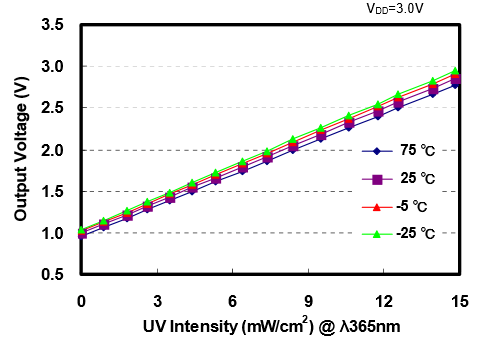
\includegraphics[scale=0.4]{2_Beschreibung_des_CANSAT/graph_photodiode_response.png}
	\caption{Spannungsausgabe vs. UV Intensität}
	\label{graph photodiode}
\end{figure}


\paragraph{Sharp Feinstaubsensor}
Der Sharp Feinstaubsensor arbeitet, wie der ML8511, sehr simpel. Im Inneren befindet sich eine Infrarot Diode, welche die Partikel anstrahlt. Auf der anderen Seite befindet sich ein Fototransistor welcher dann feststellt, wie viel von diesem Licht von Partikeln reflektiert wird, diese Veränderung ist messbar.

\begin{figure}[h]
	\centering
	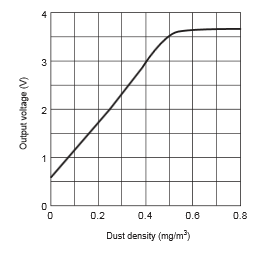
\includegraphics[scale=0.5]{2_Beschreibung_des_CANSAT/graph_photodiode_sharp.png}
	\caption{Spannungsausgabe vs. Staub}
	\label{graph photodiode}
\end{figure}

Um den Fototransistor nicht immer ganz zu bestrahlen, ist die Infrarot Diode nicht die gesamte Zeit angeschaltet. Sie scheint lediglich für den Bruchteil einer Sekunde. Die Messung muss innerhalb dieser Zeitspanne stattfinden.

\paragraph{APC220}
Der APC220, ist ein Transciever welcher entweder senden oder empfangen kann. Der BeagleBone Black schickt den formatierten JSON String per UART an den APC220. Dieser schickt ihn über die vorher am Computer festgelegte Frequenz in den Raum weiter. Am Boden befindet sich ebenfalls ein APC220, welcher die Daten empfängt.

\paragraph{Ultimate GPS}
Der Ultimate GPS von Adafruit verbindet sich mit den allgemeinen GPS-Satelliten und sendet Serial seine Daten im NMEA Format aus. Dieses Format gibt es in diversen Varianten, es verfügt aber in so gut wie allen Varianten über folgende Daten:
\begin{table}[H]
  \centering
    \begin{tabular}{rr}
    \toprule
    \textbf{Nummer} & \textbf{Daten} \\
    \midrule 
    1 & Breitengrad \\
    2 & Längengrad \\
    3 & Zeit \\
    4 & GPS-Qualität \\
    5 & Anzahl benutzter Satelliten \\
    6 & Höhe \\
    \bottomrule
    \end{tabular}
    \caption{Auslesebare Daten}
\end{table}

Außerdem können wir den Ultimate GPS über die serielle UART Schnittstelle konfigurieren um ihn zum Beispiel nur ein bestimmtes NMEA Format ausgeben zu lassen oder um die Bitrate der seriellen Übertragung zu ändern.

\paragraph{TMP006}
Der TMP006 ist ein Infrarot Temperatur Sensor, welcher die Temperatur von einem Objekt misst ohne in direktem Kontakt zu stehen. Der Sensor misst die Temperatur eines Objektes anhand der ausgestrahlten Energie auf Wellenlänge von 4 \textmu m bis zu 16 \textmu m. Durch die veränderte Spannung am Sensor ist eine Messung der Temperatur möglich. Je größer das Objekt ist, umso weiter entfernt muss es sich befinden, um vom Field of View des Sensors erfasst zu werden.

\begin{figure}[h]
	\centering
	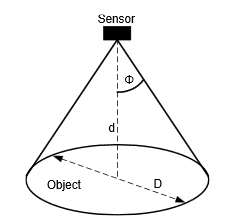
\includegraphics[scale=0.5]{2_Beschreibung_des_CANSAT/sensor_fov.png}
	\caption{Sensor Field of View}
	\label{sensor fov}
\end{figure}

Die Messung kann sehr ungenau werden, da, je nach Außentemperatur und Temperatur der Sensorfläche selber, Fehler beim Messen entstehen können.

\paragraph{BMP180}
Der BMP180 ist ein Drucksensor welcher mithilfe einer Membran den Druck misst und diesen per On-Board Controller direkt in die Höhe umrechnet. Der Sensor gibt die Daten dann per I²C-Bus aus.

\subsubsection{Energieverbrauch}
\begin{table}[H]
  \centering
    \begin{tabular}{rrrl}
    \toprule
    \textbf{Bauteil} & \textbf{Stromaufnahme} & \textbf{Spannung} & \textbf{Leistungsaufnahme} \\
    \midrule
    Beaglebone Black  & 500mA & 5V & 2500mW \\
    ML8511& <1mA & 3.3V & <3.3mW \\
    TMP006& <1mA& 3.3V& <3.3mW \\
    Sharp& 20mA & 3.3V& 66mW\\
    BMP180& <1mA& 3.3V& <3.3mW \\
    Ultimate GPS Modul& 25mA&3.3V& 82.5mW \\
    APC220& 35mA & 5V & 175mW\\

    \bottomrule
     & & &2833.4mW \\
    \bottomrule
    \end{tabular}%
    \caption{Energieverbrauch}
  \label{tab:budgetausgaben}%
\end{table}%
